\chapter{Electric Vehicles}
\label{ch:elvehicles}
% ##################################################################################################################

\hfill \textbf{Author:} Rashid A. Waraich, Joschka Bischoff

\begin{center} 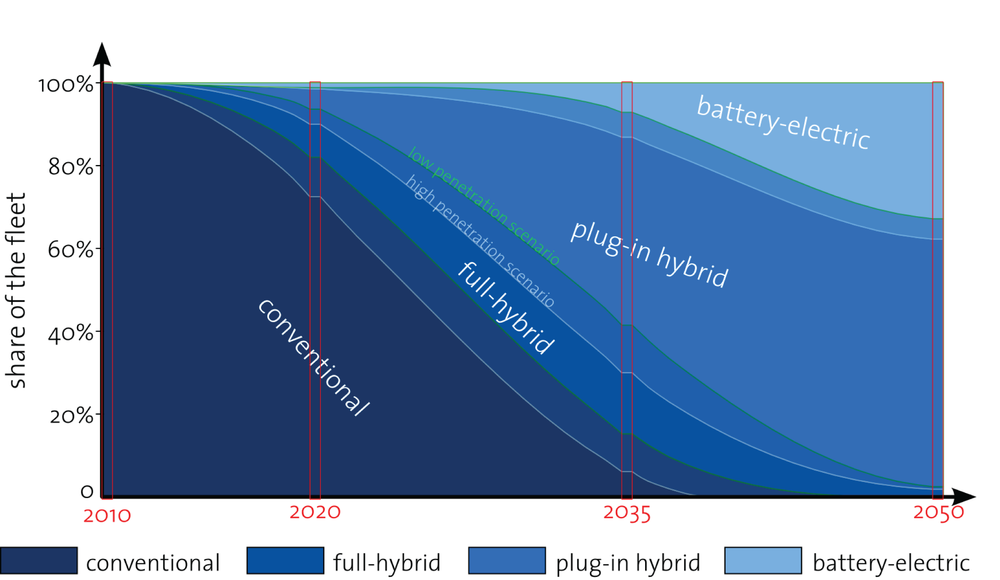
\includegraphics[width=0.65\textwidth, angle=0]{extending/figures/Elvehicles/main.png} \end{center}

\createStandardInformationBasic{transEnergySim}{No predefined invocation. A starting point is \lstinline|RunTransEnerySimExample| class}{No typical \gls{matsim} config}{\citet[][]{WaraichEtAl_TRR_2013, GalusEtAl_STRC_2009, WaraichEtAl_IATBR_2009, GalusEtAl_ITSG_2012, Waraich_PhDThesis_2014, AbedinWaraich_TechRep_IVT_2013, WaraichEtAl_TechRep_IVT_2013, GalusEtAl_ResRep_EWZ_2012, Waraich_unpub_EURO_2012, Waraich_unpub_MATSimUserMeeting_2012, WaraichEtAl_JanssensEtAl_2014, WaraichAxhausen_SDEWES_2013}}
\joschka{Verwende basic, da es kein config-basiertes Modul ist.}
% ##################################################################################################################
\section{Introduction}
The research related to \gls{ev} modeling in \gls{matsim} started in 2008/2009, within a project related to electricity grids \citep[][]{WaraichEtAl_IATBR_2009, WaraichEtAl_TRR_2013}. The goal of the project was to uncover potential bottlenecks/constraint violations in the lower voltage grid in the city of Zürich due to future \gls{ev} charging. Out of this research, a framework for \gls{ev} modeling emerged, called \gls{tesf} \citep[][]{WaraichEtAl_JanssensEtAl_2014}. This has resulted in various extensions of this framework and has allowed for simulation of various scenarios \citep[][]{WaraichEtAl_JanssensEtAl_2014, Waraich_PhDThesis_2014, AbedinWaraich_JSDEWES_2014, Schieffer_MastersThesis_2011, GalusAndersson_CIGRE_2011, GalusEtAl_ResRep_EWZ_2012, Bischoff2013MaTaxis, BischoffMaciejewskiEcabMielecMobilTUM}. This chapter gives a few pointers in these research directions and serves as a starting point for modeling \glspl{ev} in \gls{matsim}.

% ##################################################################################################################
\section{Models}
The main objective for modeling \glspl{ev} in \gls{tesf} is simple: One needs to keep track of the state of charge of the batteries in the \glspl{ev}. This means that as the \gls{ev} is driving, the depletion of the batteries is simulated. Furthermore, also the charging process of \glspl{ev} at charging infrastructure should be considered.

While the basic mechanisms of \gls{ev} modeling are simple, there are many details, when it comes to modeling scenarios. The \gls{tesf} framework provides both interfaces and implementations to cope with more complex cases, e.g., defining a vehicle which can charge contact less while driving, for example, by using dynamic inductive charging. Furthermore, also the charging mechanisms themselves can be quite complex. The following sections provides some details in this regard and the different models involved.

% ==============================================================================================
\subsection{Energy Consumption Model}
When defining a vehicle in \gls{tesf}, it can be assigned an energy consumption model, which defines how much energy the vehicle will use as driving. While for conventional vehicles just their energy consumption can be logged using such a model, for electric vehicles the energy consumption model is used to update the state of charge of the on-board battery system. \glspl{phev} can use both electricity and gasoline for driving and therefore have two different energy consumption models assigned to them for modeling these two modes. At the time of this writing, a series hybrid model has been implemented in \gls{tesf} \citep[][]{Chan_PIEEE_2007}, which uses electricity as long as the state of charge of the battery is above a certain threshold value and switches afterward to gasoline. This type of vehicle can also be charged using a plug, like a battery electric vehicle. For \glspl{phev} often car manufacturers define rules when a vehicle should switch between battery and gasoline use. The \gls{tesf} framework provides interfaces and examples of how more advanced control strategies for \glspl{phev} can be implemented.

% ==============================================================================================
\subsection{Charging Infrastructure}
Besides plug-based charging infrastructure, also inductive charging infrastructure is modeled in \gls{tesf}. There are two types of such infrastructure: A dynamic and a stationary one. The dynamic inductive charging infrastructure is often embedded in roads and vehicles which have the capability to use such infrastructure, can charge as they are driving. Stationary inductive charging is more or less the same in terms of modeling as charging using a plug, however the charging interfaces between vehicle and the charging infrastructure must match for the charging process to function.

Another approach to get a full battery quickly, is to replace/swap the used battery with a new one at specialized infrastructure, sometimes referred to as a swapping station \citep[][]{LiEtAl_ACC_2011}. A basic implementation for modeling this approach is provided in \gls{tesf}, which can be extended and detailed further according to specific scenario needs.

% ==============================================================================================
\subsection{Charging Schemes}
When an \gls{ev} connects for charging to any type of charging infrastructure, a charging scheme is needed which defines how the charging of the vehicle should operate, e.g., should the vehicle start charging immediately, or should charging happen according to pricing preferences of the agent, which may depend on time and location. Also negotiation between the vehicle computer and the grid operator may happen, which may allow for some temporal flexibility for the electricity grid, while charging a vehicles battery fully before departure (sometimes referred to as "smart charging"). Various types of such charging schemes are part of the \gls{tesf} framework and can be used to model other more complex charging schemes. Examples of various charging schemes which have been simulated with \gls{tesf} can be found in \citet[][]{WaraichEtAl_TRR_2013}.

% ==============================================================================================
\subsection{\protect\gls{v2g}}
Often in connection with electric vehicles, not only charging of vehicles is of interest, but also \gls{v2g} applications, where batteries in electric vehicles supply power and energy back to the grid \citep[][]{KemptonTomic_JPS_2005}. While the integration of \gls{v2g} models for \gls{matsim} is limited at the moment, an applications related to \gls{v2g} and intermittent energy generation at wind parks using \gls{matsim} can be found in \citet[][]{GalusAndersson_CIGRE_2011} and a preliminary attempt to integrate \gls{v2g} in \gls{tesf} is described in \citet[][]{WaraichEtAl_JanssensEtAl_2014, Schieffer_MastersThesis_2011}.

% ==============================================================================================
\subsection{Vehicle Choice}
When conducting studies related to electric vehicles, one often needs to assign each person owning a vehicle a specific type of vehicle, e.g., electric vehicle, convention vehicle, plug-in hybrid, etc. Sometimes such assignments are done at random, while ensuring vehicle type share constraints for the scenario \,\citep[e.g.,][]{WaraichEtAl_JanssensEtAl_2014}. However, often one wants to evaluate possible implications of financial or infrastructural incentives, e.g., different toll prices, parking fees or fuel prices for different types of vehicles. A replanning module for vehicle choice has been implemented recently, which also covers \glspl{ev}. First results for this are planned for publication soon and hopefully this can also be integrated in \gls{tesf} in future.

In this section an overview of the various part of the \gls{tesf} framework has been provided. In the following section an application of an extension of \gls{tesf} is given, where modeling of electric taxis is presented.

% ##################################################################################################################
\section{Application: Electric Taxis} % Author: Joschka Bischoff
A combination and extension of both the \gls{tesf} and the \gls{vrp} contribution (see Chapter~\ref{ch:dts}) allows the simulation of taxi fleets constituting of \glspl{bev}.
On the electric vehicle side, charging process of vehicle is adapted, whereas on the taxi side the concept of taxi ranks and a modified optimizer that sends idling taxis to the rank and only dispatches vehicles with a sufficient battery state of charge are introduced. 

% ==============================================================================================
\subsection{Taxi Ranks}
After dropping off a passenger, taxis proceed to the nearest rank location, unless there is an immediate follow-up request. At the rank location a queuing takes place, i.e.,\,the taxi that has arrived first will leave the rank the soonest. Other types of queuing have also been tested, e.g., a dispatch by battery \gls{soc}.
Ranks are not necessarily mandatory, however driving to them in between trips resembles a typical taxi driver behavior in Germany.

% ==============================================================================================
\subsection{Charging Process}
Chargers may be located at taxi ranks or any other link. Following any given \lstinline$AgentArrivalEvent$ of a \gls{bev} at a charger location link, charging will commence if
%
\begin{compactitem}
	\item There is a free charging spot.
	\item The vehicle's \gls{soc} is under a certain threshold.
	\item at least two minutes of time have passed that would be required for parking the car and plugging it in.
\end{compactitem}

So far, the simulation of electric taxis has been used in Mielec, Poland \citep[][]{Bischoff2013MaTaxis, BischoffMaciejewskiEcabMielecMobilTUM}. At the time of writing, an application for Berlin is in progress.

% ##################################################################################################################
\section{Usage}
The transEnergySim \gls{contribution} contains many of the features described above. Furthermore, many interfaces are provided for extending the framework and also examples are given, how different scenarios can be setup (e.g., energy consumption model, vehicle types, charging schemes, etc.).

% ##################################################################################################################

